\documentclass[a4paper]{article}
\usepackage[printsolution=false]{exercises}
\usepackage{url}
\usepackage{background, hyperref}
\usepackage{tcolorbox}
\usepackage{lastpage}
\usepackage{fancyhdr}
\usepackage{xcolor}
\usepackage[sfdefault]{cabin}
\usepackage{graphicx}
\usepackage[T1]{fontenc}
\usepackage[backend=bibtex,style=authoryear,natbib=true]{biblatex}
\addbibresource{points.bib}

\pagestyle{fancy}
\fancyhead[L,C,R]{}
\fancyfoot[L]{\small CTDS workshop, Univ. of St Andrews}
\fancyfoot[R]{\small Practical 1 - point transects}
\fancyfoot[C]{\small \thepage\ of \pageref{LastPage}}
\renewcommand{\headrulewidth}{0pt}
\renewcommand{\footrulewidth}{1pt}

\newif\iffirstpage
\firstpagetrue
\backgroundsetup{contents={%
 			\iffirstpage
				\includegraphics[width=\textwidth]{jaguar1.jpg}%
				\global\firstpagefalse
				\fi
			},
			scale=1,placement=top,opacity=0.6,position=current page.north, vshift=-1cm
}

\begin{document}
%% don't mess with blank lines here in the title.
\phantom{a}

\bigskip

{\Large Camera trap distance sampling workshop}

{\large 21-25 March 2022}

\begin{flushright}
\tiny{Source: \url{https://unsplash.com/@satyadeep_d}}
\end{flushright}

\ifsolutionthenelse{%
{\Large \color{blue}Solution \\}
{\color{blue}\rule{\linewidth}{0.5mm}}
}%
{%
}

In this exercise you will analyse point transect survey data: camera trap data are a special case of point transect sampling. This practical acquaints you with fitting detection functions to point transect data. In the first problem, the data are simulated and so the true density is known. In the second problem, two different data collection methods were used to survey song birds.

\section{Simulated data}
Simulated point transect data from 30 points are given in the data set PTExercise. These data were generated from a half-normal detection function and the true density was 79.8 animals/hectare.  The radial distances were recorded in metres. Although the data were simulated with exact distances to each detection, we are going to analyze the data as if it were collected in equally-spaced 2.5m distance bins, because binned (also called ``interval’’) data are the norm in camera trap surveys.

\subsection{Fit a half normal detection function}

\subsubsection{Examine the fit of the model to the data}
Through both formal goodness-of-fit test and visually via plotting

\subsection{Experiment with other models}
\begin{itemize}
	\item Experiment with keys other than the half normal (i.e. hazard rate and uniform) to assess whether these data can be satisfactorily analysed using the wrong model:
		\begin{itemize}
		  \item determine a suitable truncation distance, and
		  \item for each key function decide whether any adjustments are needed.
		\end{itemize}
	\item How do the bias and precision compare between models?
\end{itemize}

Note, to define a different truncation distance, you can change the upper limit of the cutpoints sequence – for example, to define a truncation distance of 30m.

\ifsolutionthenelse{%

	\begin{tcolorbox}[colback=green!5!white, colframe=green!60!black, title=Simulated point transect data]

From the table of model results below, note the following:
\begin{itemize}
	\item Hazard rate key least favoured, but half normal and uniform cosine compete for most favoured
	\item Estimates from uniform cosine model and hazard rate model change considerably as a result of truncation; half normal model much less so
	\item For a given truncation value, there is considerable variation in density estimates between models.
		\begin{itemize}
			\item Using 22.5m truncation as an example, the largest density estimate is 1.3 times greater than the smallest density estimate.
		\end{itemize}
\end{itemize}

Therefore model selection is more influential in density estimation for point transect surveys than for line transect surveys.

{\small
\begin{tabular}{lrrrrrr}
Model                        & params & $\Delta$ AIC & D     & D LCL & D UCL  & D CV \\
\hline
halfnorm cosine no trunc     & 1         & 1.17      & 80.98 & 63.46 & 103.33 & 0.12 \\
hazard hermite no trunc & 2         & 3.66      & 49.23 & 38.97 & 62.18  & 0.12 \\
uniform cosine no trunc & 2         & 0.00      & 73.88 & 60.16 & 90.72  & 0.10 \\
\hline
halfnorm cosine trunc 27.5   & 1         & 0.00      & 78.59 & 61.01 & 101.24 & 0.13 \\
hazard hermite trunc 27.5    & 2         & 2.70      & 51.36 & 40.18 & 65.65  & 0.12 \\
uniform cosine trunc 27.5    & 1         & 0.03      & 64.24 & 53.09 & 77.73  & 0.09 \\
\hline
halfnorm cosine trunc 22.5   & 1         & 0.71      & 78.47 & 59.33 & 103.78 & 0.14 \\
hazard hermite trunc 22.5    & 3         & 0.48      & 62.04 & 47.09 & 81.74  & 0.14 \\
uniform cosine trunc 22.5    & 3         & 0.00      & 82.24 & 49.22 & 137.41 & 0.26 \\
\hline
halfnorm cosine trunc 20     & 1         & 0.00      & 71.54 & 52.56 & 97.38  & 0.16 \\
hazard hermite trunc 20      & 2         & 2.95      & 61.36 & 42.53 & 88.51  & 0.19 \\
uniform cosine trunc 20      & 1         & 1.34      & 75.55 & 57.17 & 99.83  & 0.14
\end{tabular}
}
\end{tcolorbox}
}%
{%
}

\section{Songbird point transect data}

A point transect survey of songbirds was conducted at Montrave, Fife, Scotland, in 2004 \citep{buckland2006} and for this exercise, the data gathered from winter wrens is used. Several different methods of data collection were used and for this exercise, two point transect methods are used:

\begin{itemize}
    \item standard five-minute counts and
    \item the ‘snapshot’ method.
\end{itemize}

For each method the same 32 point transects were used in 33.2 ha of parkland (Figure 1) and each point transect was visited twice. Detection distances (recorded in metres) were measured with the aid of a rangefinder.

\begin{figure}
\centering
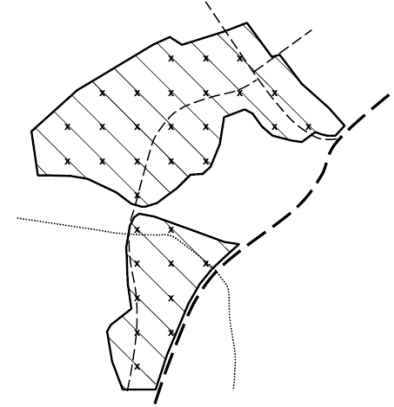
\includegraphics[scale=0.5]{Prac_5_Figure_1.png}
\caption{The study site at Montrave in Fife, Scotland. The dotted line is a small stream, the thin dashed lines are tracks, and the thick dashed line a main road. The 32 points are shown by crosses, and are laid out on a systematic grid with 100m separation.}
\end{figure}

Note the Effort field is 2 meaning each point transect was visited twice.

Although the data were collected using exact distances, we will again assume they were collected in distance bins, to make things more comparable with our future camera trap analyses. We will assume 10m distance bins out to 40m and then 20m bins thereafter; in both datasets the maximum distance is 120m. Adjust the analysis such that bins are used, setting 8 cutpoints to create 7 distance bins as in the screen shot below:

\begin{figure}
\centering
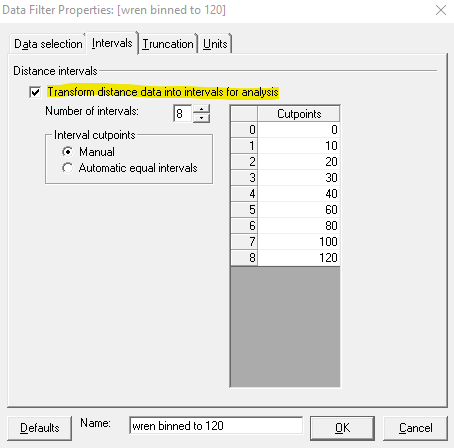
\includegraphics[scale=0.5]{DistWingrabs/transform-to-bins.png}
\end{figure}

\subsection{Analyses to perform}

\begin{itemize}
	\item Start with a simple model for exploration.
	\begin{itemize}
		\item Experiment with truncation distances $w$ and choose a value of $w$ for each data set
		\item Are there any troubling issues in either data set?
	\end{itemize}
\ifsolutionthenelse{%
	\begin{tcolorbox}[colback=red!5!white, colframe=red!60!black, title=Possible problem in the data?]
		 There is some reason to suspect evasive movement.  This can be seen when looking at the $\chi^2$ goodness of fit test.  There are fewer detections than the model would predict in the first three intervals and more detections than the model would predict in bins four and five.  The model does still fit the data.
		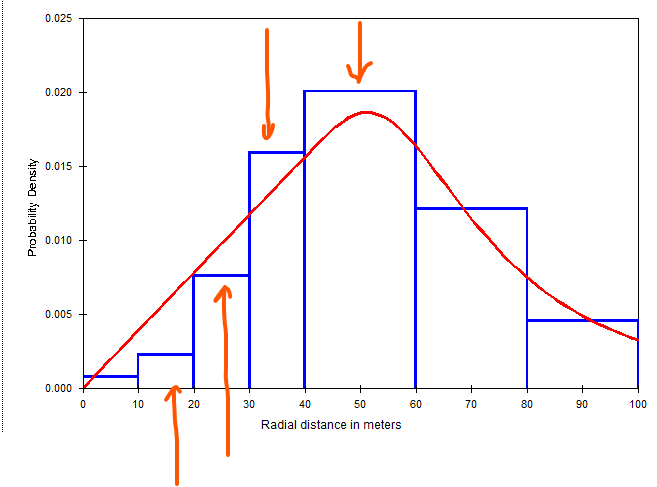
\includegraphics[scale=0.5]{DistWingrabs/evasivemovement.png}
	\end{tcolorbox}
}%
{%
}

	\item Try some other models (key functions and adjustement)
	\item From AIC scores, plots and goodness-of-fit statistics, choose an adequate model
	\item Record point and interval estimates for your chosen model of each data set.
\end{itemize}

Territory mapping of winter wrens in this study area suggested territory density of 1.30 $territories^{-1}$

\ifsolutionthenelse{%

	\begin{tcolorbox}[colback=green!5!white, colframe=green!60!black, title=Remarks about analysis of the 5 minute wren analysis]
		\begin{itemize}
			\item There is little effect of truncation of the most distant bin upon the point estimate of density for any of the key function models
			\item The hazard rate key found no use for adjustment terms to improve its fit (with or without truncation
			\item In contrast, the half normal found the need for two adjustment terms in both instances.  The result is a three parameter model
			\begin{itemize}
				\item Look at the resulting loss of precision in the density estimates
			\end{itemize}
			\item As an aside, look in detail at the result of the uniform key with cosine adjustment in the no truncation case.  That model did not converge.
		\end{itemize}
%\begin{table}[h]
{\small
\begin{tabular}{lrrrrrrrr}
Model   &  params & $\Delta$ AIC & D        & D LCL     & D UCL    & D CV         \\
\hline
hn cos no trunc       & 3        & 2.53  & 1.27 & 0.58 & 2.78 & 0.41\\
haz hermite no trunc  & 2        & 0     & 1.24 & 0.97 & 1.58 & 0.12\\
unif cosine no trunc  & 1        & 6.41  & 1.56 & 1.28 & 1.89 & 0.10\\
\hline
hn cos trun100        & 3        & 2.53  & 1.32 & 0.58 & 3.00 & 0.43\\
haz hermite trunc 100 & 2        & 0     & 1.28 & 0.98 & 1.69 & 0.14\\
unif cosine trunc 100 & 2        & 2.98  & 1.43 & 0.89 & 2.28 & 0.24   
\end{tabular}
}
%\end{table}
\end{tcolorbox}

%=====================================================
	\begin{tcolorbox}[colback=green!5!white, colframe=green!60!black, title=Remarks about analysis of the snapshot wren analysis]
	\begin{itemize}
		\item Note the hazard rate model is preferred by AIC.  However, this model predicts perfect detectability of wrens to a distance of 50-60m from the point.  The person responsible for collecting these data suggested this is improbable and chose to make inference from a model different that the one preferred by AIC.  In his words "a model with a slightly higher AIC value and a more plausible fit to the detection function was selected." Goodness of fit deteriorates a bit, but is still acceptable.
		\item Note too the cost (in terms of precision) of the adjustment terms added to the half normal key function for both truncation levels.
	\end{itemize}

{\small
\begin{tabular}{lrrrrrr}
Name                      & params & $\Delta$ AIC & D    & D LCL & D UCL & D CV \\
\hline
halfnorm cosine no trunc  & 3      & 2.67      & 1.11 & 0.49  & 2.53  & 0.43 \\
hazard hermite no trunc   & 2      & 0.00      & 1.07 & 0.85  & 1.34  & 0.12 \\
uniform cosine no trunc   & 1      & 5.05      & 1.37 & 1.15  & 1.64  & 0.09 \\
\hline
halfnorm cosine trunc 100 & 3      & 3.08      & 1.15 & 0.48  & 2.74  & 0.46 \\
hazard hermite trunc 100  & 2      & 0.00      & 1.08 & 0.84  & 1.38  & 0.13 \\
uniform cosine trunc 100  & 2      & 3.19      & 1.25 & 0.76  & 2.04  & 0.25
\end{tabular}
}
	\end{tcolorbox}

}%
{%
}

\printbibliography

\end{document}